\documentclass[conference]{IEEEtran}

\ifCLASSINFOpdf
   \usepackage[pdftex]{graphicx}
  % declare the path(s) where your graphic files are
  % \graphicspath{{../pdf/}{../jpeg/}}
  % and their extensions so you won't have to specify these with
  % every instance of \includegraphics
   \DeclareGraphicsExtensions{.pdf,.jpeg,.png}
\else
  % or other class option (dvipsone, dvipdf, if not using dvips). graphicx
  % will default to the driver specified in the system graphics.cfg if no
  % driver is specified.
   \usepackage[dvips]{graphicx}
  % declare the path(s) where your graphic files are
  % \graphicspath{{../eps/}}
  % and their extensions so you won't have to specify these with
  % every instance of \includegraphics
   \DeclareGraphicsExtensions{.eps, .ps}
\fi

\hyphenation{}


\begin{document}

\title{}

% author names and affiliations
% use a multiple column layout for up to three different
% affiliations
\author{\IEEEauthorblockN{Mads Ruben Burgdorff Kristensen}
\IEEEauthorblockA{eScience Centre\\
University of Copenhagen\\
Denmark}
\and
\IEEEauthorblockN{Brian Vinter}
\IEEEauthorblockA{eScience Centre\\
University of Copenhagen\\
Denmark}}

% make the title area
\maketitle

\begin{abstract}

\end{abstract}

\IEEEpeerreviewmaketitle

\section{Introduction}

\subsection{Motivation}

\section{Data Layout}
\begin{figure}
 \centering
 \includegraphics[width=\linewidth]{gfx/datalayout}
 \caption{The Two-Dimensional Block Cyclic Distribution of a matrix on a 2 x 3 grid of processors.}
 \label{fig:datalayout}
\end{figure}

Two-Dimensional Block Cyclic Distribution is a very popular distribution scheme and it is used in numerical libraries like ScaLAPACK\cite{Blackford96} and LINPACK\cite{linpack79}. It supports matrices and vectors and has a good load balance in numerical problems that have a diagonal computation workflow e.g. Gaussian elimination. The distribution scheme works by arranging all MPI-processes in a two dimensional grid and then distributing data-blocks in a round-robin fashion either along one or both grid dimensions (Fig. \ref {fig:datalayout}); the result is a well-balanced distribution.

NumPy is not limited to matrices and vectors as it supports arrays with an arbitrary number of dimensions. DistNumPy therefore use a more generalized N-Dimensional Block Cyclic Distribution inspired by High Performance Fortran\cite{Loveman93}, which supports an arbitrary number of dimensions. Instead of using a fixed process grid, we have a process grid for every number of dimensions. This works well when operating on arrays with the same number of dimensions but causes problems otherwise. For instance in a matrix-vector multiplication the two arrays are distributed on different process grid and may therefore require more communication. ScaLAPACK solves the problem by distributing vectors on two-dimensional process grids instead of one-dimensional process grids, but this will result in vector operations that cannot utilize all available processors. An alternative solution is to redistribute the data between a series of identically leveled BLAS operations using a fast runtime redistribution algorithm like \cite{PrylliT97} demonstrates.


\begin{figure}
 \centering
 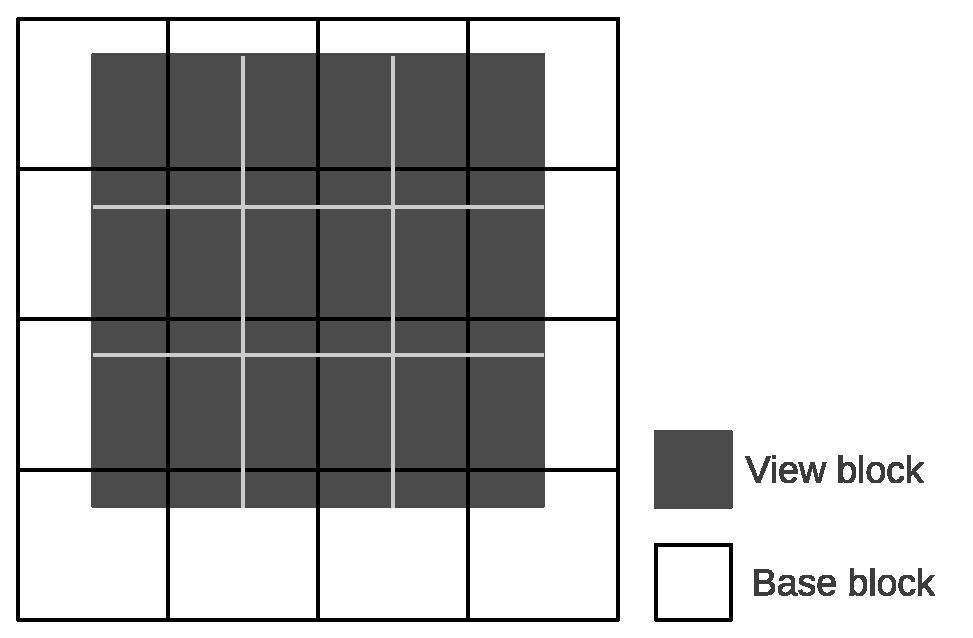
\includegraphics[width=150px]{gfx/view_blocks}
 \caption{}
 \label{fig:view_block}
\end{figure}






\bibliographystyle{IEEEtran}
\bibliography{/home/madsbk/repos/priv/diku/phd/paper_archive/main}

\end{document}